\documentclass{class/report}

\title{ACPCE Transactional System Using OAuth 2.0}
\reportstage{1}
\degree{Bachelor of Engineering}
\degreespecialization{Computer Engineering}
\department{Department of Computer Engineering}
\academicyear{2014}{2015}
\hod{Prof. R. C. Suryawanshi}
\principal{Dr. V. N. Pawar}
\guide{Dr. M. M. Despande}
\coguide{Prof. S. P. Bansu}
\author{Jaiesh Bhagat (151041042)}
%\coauthor{Pratul Sutar (151041042)}
\declarationdate{Wednesday}{22\textsuperscript{nd} March, 2020}
\declarationplace{Navi Mumbai, Maharashtra}

\begin{document}

\maketitle

\begin{dedication}
To my college...
\end{dedication}

\makecertificate

\makedeclaration

\begin{abstract}
This report specifies the various processes and techniques used in gathering requirements, designing, implementing and testing for the project on ‘ACPCE Transactional System Using OAuth 2.0’. Existing problems with current system in the institute was analysed and noted. This project aims to solve some of the problems by creating a core software, development platforms for future works and to set up necessary infrastructure for maintaining transactional data for the institute, thus, adding more value to the current system. The requirements were gathered from various institute departments and stakeholders, based on which, requirement was modelled. A web application, using Java, MySQL and frameworks like Spring, Hibernate, Apache, etc, was designed to fulfil the modelled requirements. Features of the system includes, but are not limited to, Admissions, Student and Staff Dashboard, Examinations, Results, WebAdmin, ACPCE SSO and Attendance.
\end{abstract}

\tableofcontents
 
\listoffigures
 
\listoftables

\chapter{Introduction}
Transaction processing is a way of computing that divides work into individual, indivisible operations, called transactions. A transaction processing system (TPS) is a software system, or software/hardware combination, that supports transaction processing.
\par
A transaction process system (TPS) is an information processing system for business transactions involving the collection, modification and retrieval of all transaction data. Characteristics of a TPS include performance, reliability and consistency.
\par
TPS is also known as transaction processing or real-time processing. Transaction systems must be able to support a high number of concurrent users and transaction types.
\par
 \ref{fig:oltp} shows the main characteristics of a transaction system. Before the advent of the Internet, a transaction system served hundreds or thousands of terminals with dozens or hundreds of transactions per second. This workload was rather predictable both in transaction rate and mix of transactions.
 \begin{figure}[ht]
\centering
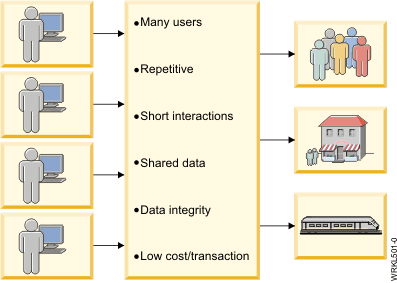
\includegraphics[width=25em]{figures/figure1.png}
\caption{Characteristics of Transactional Systems}
\label{fig:oltp}
\end{figure}
\par

Transaction systems must be able to support a high number of concurrent users and transaction types.
\par
One of the main characteristics of a transaction or online system is that the interactions between the user and the system are very brief. Most transactions are executed in short time periods--one second, in some cases. The user will perform a complete business transaction through short interactions, with immediate response time required for each interaction. These are mission-critical applications; therefore, continuous availability, high performance, and data protection and integrity are required.
\par
Online transaction processing (OLTP) is transaction processing that occurs interactively; it requires:
\begin{itemize}
\item Immediate response time
\item Continuous availability of the transaction interface to the end user
\item Security
\item Data integrity.
\end{itemize}
Online transactions are familiar to many people. Some examples include:
\begin{itemize}
\item ATM transactions such as deposits, withdrawals, inquiries, and transfers
\item Supermarket payments with debit or credit cards
\item Buying merchandise over the Internet.
\end{itemize}
\par
In fact, an online system has many of the characteristics of an operating system:
\begin{itemize}
\item Managing and dispatching tasks
\item Controlling user access authority to system resources
\item Managing the use of memory
\item Managing and controlling simultaneous access to data files
\item Providing device independence.
\end{itemize}
\par
Transactional systems are databases that record a company’s daily transactions. The three major transactional databases include CRM (customer relationship management), HRM (human resources management), and ERP (enterprise resource planning). For instance, a sales transaction would be recorded and stored as a piece of data in the CRM database.
\par
Transactional systems are not considered optimal for business intelligence. This is for a variety of reasons, including the fact that a) data is not optimized for reporting and analysis and b) querying directly against these databases may slow down the system and prevent the databases from recording transactions in real time.
\par
In some cases, companies use an ETL tool to collect data from their transactional databases, transform them to be optimized for BI, and load them into a data warehouse or other data mart. The main downside of this approach is that a data warehouse is a complex and expensive architecture, which is why many other companies opt to report directly against their transactional databases.
\par
A transaction process system and transaction processing are often contrasted with a batch process system and batch processing, where many requests are all executed at one time. The former requires the interaction of a user, whereas batch processing does not require user involvement. In batch processing the results of each transaction are not immediately available. Additionally, there is a delay while the many requests are being organized, stored and eventually executed. In transaction processing there is no delay and the results of each transaction are immediately available. During the delay time for batch processing, errors can occur. Although errors can occur in transaction processing, they are infrequent and tolerated, but do not warrant shutting down the entire system.
\par
To achieve performance, reliability and consistency, data must be readily accessible in a data warehouse, backup procedures must be in place and the recovery process must be in place to deal with system failure, human failure, computer viruses, software applications or natural disasters.
\par
\section{Objectives}
Objective of the system is to provide a better solution to manage college activities in an efficient manner and increase the productivity of the system.
\begin{enumerate}
\item To convert all offline process into online.
\item Improve service experience.
\item Less maintenance cost and time saving.
\item Development of Software Development Kit (SDKs) for future developments.
\item Designing of API based architecture to achieve maximum cross-compatibility.
\end{enumerate}
\section{Project Scope}
Expectations for improved performance are always increasing, higher education leaders continue to think more creatively about how their people, process and technology can work together more efficiently. The transactional system will support this view by helping institutions build, manage and extend their digital campus. It enables individuals, systems and communities to interact seamlessly across campus in an environment where efficiency, service delivery and personalized education experiences propel desired outcomes. This project aims to convert manual procedures into an automated single software.
\chapter{Review of Literature}
Following applications from various publishers were analysed from the internet to understand the existing services available in the market.
\section{Literature Review}
\begin{longtable}[c]{| c | l |}
\hline \textbf{Service Provider} & \textbf{Review} \\
  \hline
\begin{tabular}[c]{@{}l@{}}A. C. Patil College\\ System \cite{ACPCE}\end{tabular} & \begin{tabular}[c]{@{}l@{}}Microsoft Excel, Google Spreadsheets and \\ white book is used to capture transactional data.\\ It is difficult to maintain and manage this data.\\ Currently, our college is using Ziksa ERP system to \\ carry out some activities.\end{tabular}\\\hline
EDaura \cite{EDaura} &
  \begin{tabular}[c]{@{}l@{}}EDaura is a skill-based learning environment with\\ a mobile-first approach. EDaura gives educators\\ and learners a set of tools with powerful analytics\\ and assessment to improve the educational process.\\ The value EDaura offers placing the assessment as\\ the core of the learning cycle through chat\\ communication, course classroom management\\ and content distribution.\end{tabular} \\ \hline
EduWave \cite{EduWave} &
  \begin{tabular}[c]{@{}l@{}}EduWave is the first educational platform\\
  worldwide providing all the required educational\\
  solution, LMS, SIS, CC and EMIS under one\\
  platform. The platform is delivered by cloud, on-\\
  premise, SaaS and mobile apps for Android and\\
  iOS.
\end{tabular} \\ \hline
FACTS \cite{FACTS} & \begin{tabular}[c]{@{}l@{}}Ren Web provides 300+ core features and powerful\\
integrated solutions that automate your school\\ administration, classroom management,\\
communication with the home.\\
This web-based solution offers a turnkey data\\
conversion and setup process, comprehensive\\ training and live customer support.\end{tabular} \\ \hline
\caption{Review of Popular Academic TPS} 
\end{longtable}
\section{Analysis of Review}
After reviewing the above systems, it has been analysed that almost all the systems have their own specific format. These systems are not capable to offer custom services that are specific to various institutes that are affiliated to University of Mumbai.
\par
These systems lack customizability of various parameters that are dynamically controlled by the university. With such systems, still, there will arise needs to enforce manual workflows. These systems are made as per the standard format and does not provide flexibility as per the user requirements. All the systems have almost the same modules and major emphasis is given on admissions, student-staff relation and examination.  Major moto of the system is to integrate intra college activities into a single system.  Most of the systems also provide mobile apps for students and parents.
\chapter{Description}
\section{Problem Statement}
\begin{itemize}
\item The objective of the project is to overcome the disadvantages present in the existing system.
\item Provide tailor made services to accommodate dynamic parameters of the university.
\item Provide tailor made services to the needs of institute.
\item Bridging gap between manual human work flow to digital work flow.
\end{itemize}
\section{Features of Proposed System}
\begin{itemize}
\begin{figure}[ht]
\centering
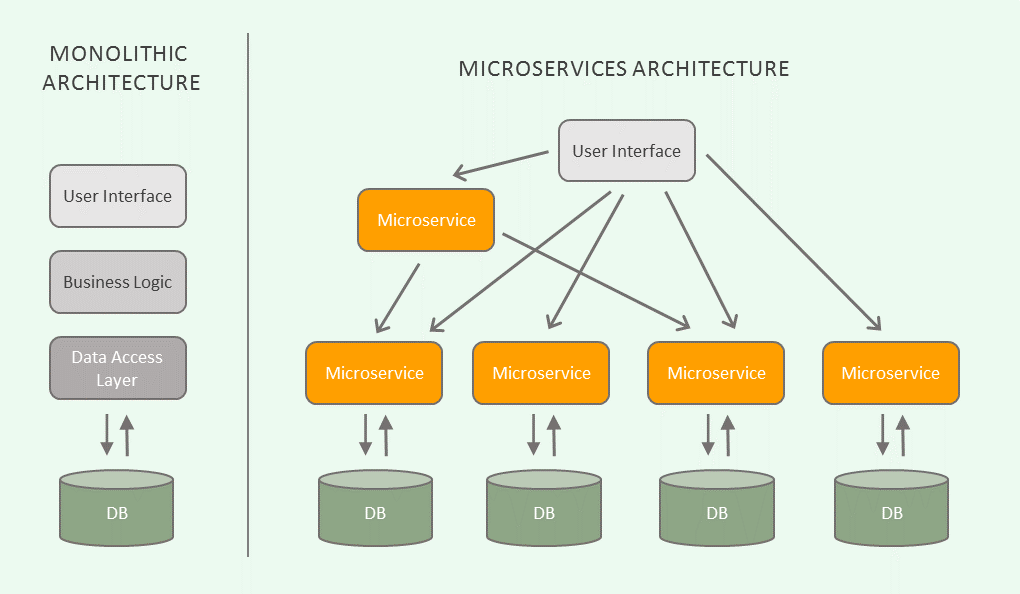
\includegraphics[width=35em]{figures/figure2.png}
\caption{Mono Lithic v/s Micro Service Architecture}
\end{figure}
\item \textbf{Microservice Architecture}\par
Microservices are a software development technique —a variant of the service-oriented architecture (SOA) structural style— that arranges an application as a collection of loosely coupled services. In a microservices architecture, services are fine-grained and the protocols are lightweight.
\begin{figure}[ht]
\centering
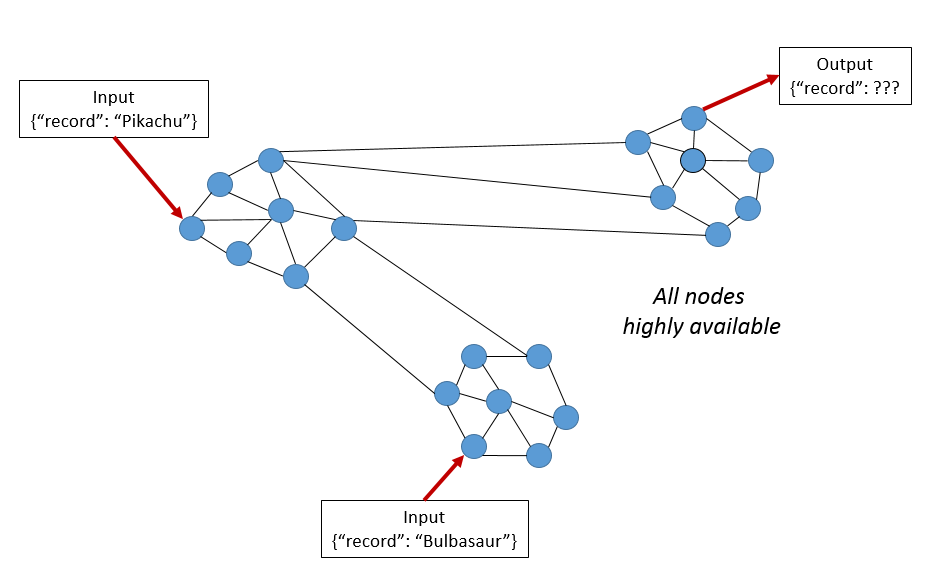
\includegraphics[width=35em]{figures/figure3.png}
\caption{Distributed System Architecture}
\end{figure}
\item \textbf{Distributed System}\par
Distributed computing is a field of computer science that studies distributed systems. A distributed system is a system whose components are located on different networked computers, which communicate and coordinate their actions by passing messages to one another. The components interact with one another in order to achieve a common goal. Three significant characteristics of distributed systems are: concurrency of components, lack of a global clock, and independent failure of components. Examples of distributed systems vary from SOA-based systems to massively multiplayer online games to peer-to-peer applications.
\par
A computer program that runs within a distributed system is called a distributed program (and distributed programming is the process of writing such programs). There are many different types of implementations for the message passing mechanism, including pure HTTP, RPC-like connectors and message queues.
\par
Distributed computing also refers to the use of distributed systems to solve computational problems. In distributed computing, a problem is divided into many tasks, each of which is solved by one or more computers, which communicate with each other via message passing.
\begin{figure}[ht]
\centering
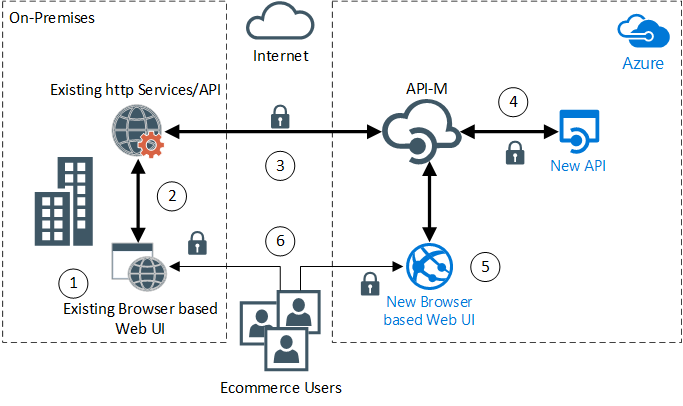
\includegraphics[width=35em]{figures/figure4.png}
\caption{API System Architecture}
\end{figure}
\item \textbf{API Oriented}\par
An application programming interface (API) is an interface or communication protocol between a client and a server intended to simplify the building of client-side software. It has been described as a “contract” between the client and the server, such that if the client makes a request in a specific format, it will always get a response in a specific format or initiate a defined action.
\par
An API may be for a web-based system, operating system, database system, computer hardware, or software library.
\par
An API specification can take many forms, but often includes specifications for routines, data structures, object classes, variables, or remote calls. POSIX, Windows API and ASPI are examples of different forms of APIs. Documentation for the API usually is provided to facilitate usage and implementation.
\item \textbf{Cross Platform Development}\par
Cross-platform software (also multi-platform software or platform-independent software) is computer software that is implemented on multiple computing platforms. Cross-platform software may be divided into two types; one requires individual building or compilation for each platform that it supports, and the other one can be directly run on any platform without special preparation, e.g., software written in an interpreted language or pre-compiled portable bytecode for which the interpreters or run-time packages are common or standard components of all platforms.
\item \textbf{Role Based Security}\par
Role-based access control (RBAC) or role-based security is an approach to restricting system access to authorized users. It is used by the majority of enterprises with more than 500 employees, and can implement mandatory access control (MAC) or discretionary access control (DAC).
\par
Role-based access control (RBAC) is a policy-neutral access-control mechanism defined around roles and privileges. The components of RBAC such as role-permissions, user-role and role-role relationships make it simple to perform user assignments.

\item \textbf{Central Identity Management}\par
Identity management system refers to an information system, or to a set of technologies that can be used for enterprise or cross-network identity management.
\par
Additional terms are used synonymously with “identity management system” including;
\begin{itemize}
\item Access governance system
\item Identity and access management system
\item Entitlement management system
\item User provisioning system
\end{itemize}
Identity management (IdM) describes the management of individual identities, their authentication, authorization, roles and privileges within or across system and enterprise boundaries with the goal of increasing security and productivity while decreasing cost, downtime, and repetitive tasks.
\par
"Identity management" and "access and identity management" (or AIM) are terms that are used interchangeably under the title of identity management while identity management itself falls under the umbrella of IT security.
\par
Identity management systems, products, applications, and platforms are commercial Identity management solutions implemented for enterprises and organizations.
\par
Technologies, services, and terms related to identity management include active directories, service providers, identity providers, Web services, access control, digital identities, password managers, single sign-on, security tokens, security token services (STS), workflows, OpenID, WS-Security, WS-Trust, SAML 2.0, OAuth, and RBAC.
\begin{figure}[ht]
\centering
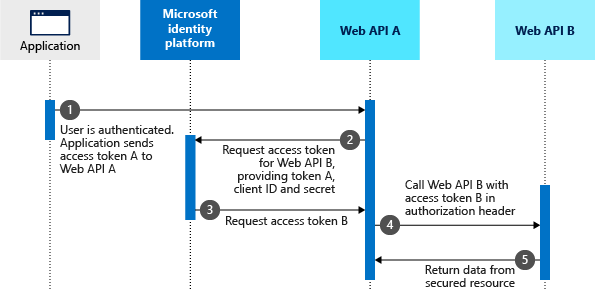
\includegraphics[width=35em]{figures/figure5.png}
\caption{OAuth 2.0 Flow}
\end{figure}
\item \textbf{Utilizes OAuth 2.0 Architecture}\par
OAuth is an open standard for access delegation, commonly used as a way for Internet users to grant websites or applications access to their information on other websites but without giving them the passwords. This mechanism is used by companies such as Amazon, Google, Facebook, Microsoft and Twitter to permit the users to share information about their accounts with third party applications or websites.
\end{itemize}
\section{Overview of Proposed System}
Capturing complete academic lifecycle of student into the system. Scopes of student’s application include:
\begin{itemize}
\item Attendance
\item Results
\item Library
\item Admissions
\item Fests
\item Availability of Staff
\end{itemize}
\par
Capturing complete journey of staff into the system. Scopes of staff’s application include:
\begin{itemize}
\item Communication
\item Attendance
\item Capture student data
\item Admissions
\item Leave Status
\item Calendar
\end{itemize}
\chapter{Design Approach}
\section{Proposed System}
A transaction server is a specialized type of server that manages the operations of software-based transactions or transaction processing. It manages application and database transactions on a network or Internet, within a distributed computing environment.
\par
A transaction server may also be referred to as a transaction processing system (TPS) or as a part of one composite TPS solution. A transaction server primarily enables transactions to be processed within distributed computing applications. Typically, a transaction server is a combination of hardware, software and network components that altogether ensures completion of each transaction. A transaction server works when an application or application server requests for a specific data object residing on a database or database server on the network or Internet. The transaction server acts as an intermediary server that can ensure that the application or user receives the requested data from the database or the completion of that transaction.
\par
The transaction server is also the name of a Microsoft Server (Viper) or Microsoft transaction server (MTS), which provides similar functionality. It provides transaction processing services on the COM/DCOM based software components.
\par
Distributed computing is a computing concept that, in its most general sense, refers to multiple computer systems working on a single problem. In distributed computing, a single problem is divided into many parts, and each part is solved by different computers. As long as the computers are networked, they can communicate with each other to solve the problem. If done properly, the computers perform like a single entity.
\par
The ultimate goal of distributed computing is to maximize performance by connecting users and IT resources in a cost-effective, transparent and reliable manner. It also ensures fault tolerance and enables resource accessibility in the event that one of the components fails.
\par
This first started with the use of data entry terminals on mainframe computers, then moved into minicomputers and is now possible in personal computers and client-server architecture with more tiers.
\par
A distributed computing architecture consists of a number of client machines with very lightweight software agents installed with one or more dedicated distributed computing management servers. The agents running on the client machines usually detect when the machine is idle and send a notification to the management server that the machine is not in use and available for a processing job. The agents then requests an application package. When the client machine receives this application package from the management server to process, it runs the application software when it has free CPU cycles and sends the result back to the management server. When the user returns and requires the resources again, the management server returns the resources was using to perform different tasks in the user's absence.
\section{Architecture}
\begin{figure}[ht]
\centering
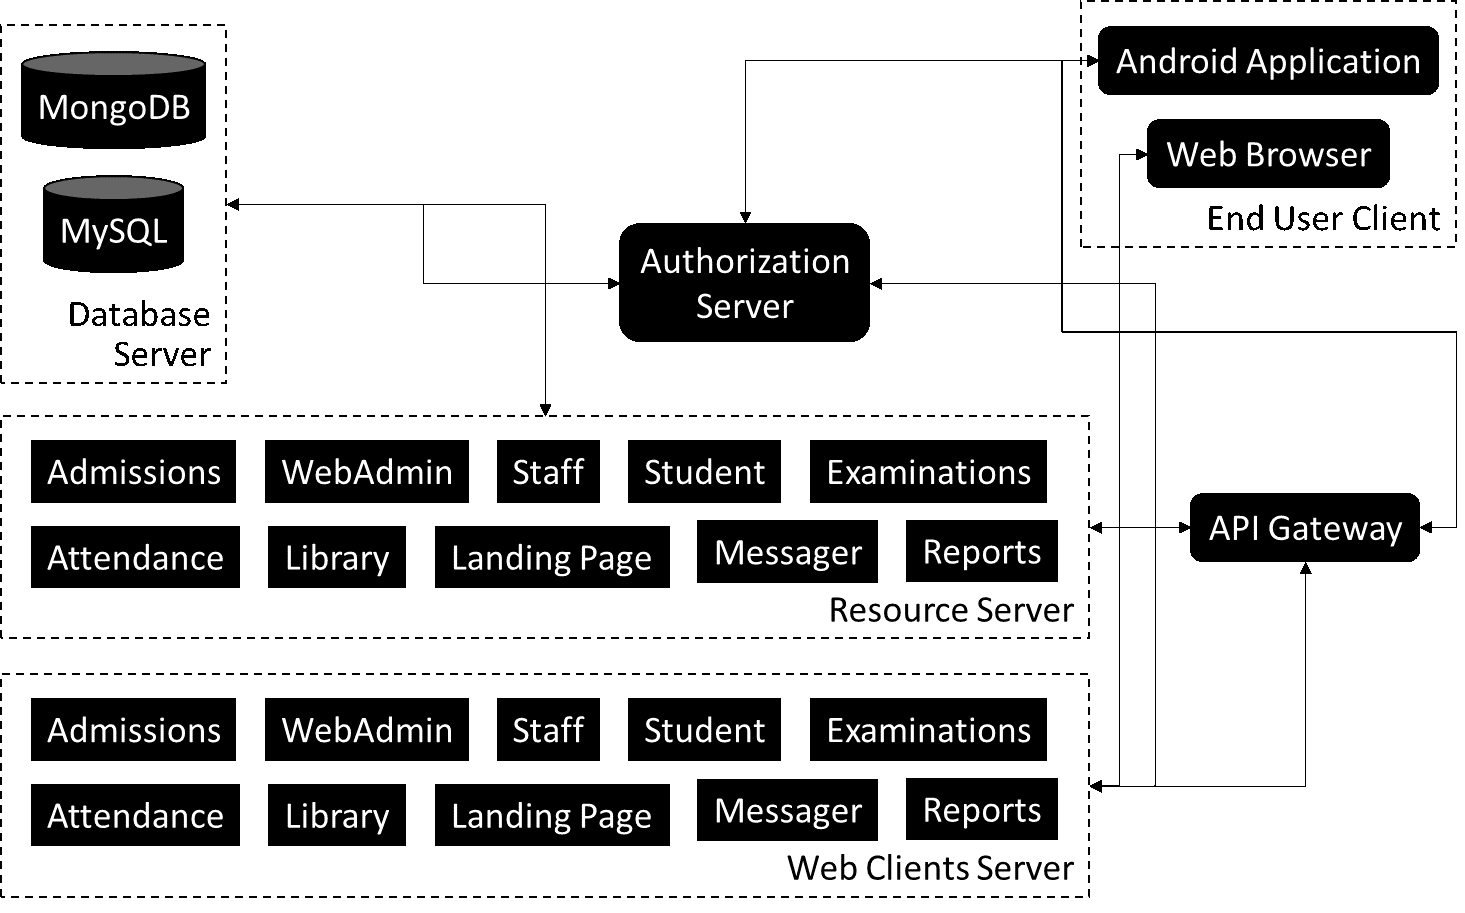
\includegraphics[width=35em]{figures/figure6.png}
\caption{OAuth 2.0 Flow}
\end{figure}
\chapter{Implementation}
\section{Code}
\lstinputlisting[language=Java, 
caption=org.acpce.model.AcpceOAuth2User
]{code/AcpceOAuth2User.java}
\lstinputlisting[language=Java, 
caption=org.acpce.model.Staff
]{code/Staff.java}
\lstinputlisting[language=Java, 
caption=org.acpce.model.Student
]{code/Student.java}
\chapter{Conclusion \& Future Work}

\bibliography{plain}{chapters/bibliography}

\makeacknowledgement

\end{document}
